\documentclass[12pt]{article}
% \usepackage[hyphens,spaces,obeyspaces]{url}

\usepackage{float} % to force the image to be where we want it
\usepackage[letterpaper, margin=1in]{geometry} 
\usepackage{graphicx}
\usepackage{hyperref}
\usepackage{amsmath}
\usepackage{amsfonts}
\usepackage{amssymb}
\usepackage[
backend=biber,
style=numeric,
sorting=none
]{biblatex}
\addbibresource{ref.bib}

\usepackage{nopageno} % Required by SIGBOVIK, no page numbers!


% For the diagram
\usepackage{tikz}
\usetikzlibrary{positioning, arrows.meta}

\title{Exploring the Viability of Utilising Multi-Modal GPT Models with Local Hardware for Image Text Detection}
\author{\href{mailto:talesfromprod+sigbovik2024@gmail.com}{Richard Finlay Tweed} MSci\\ Department of Futile Research, No Associated University}
\date{2024-03-14}

\begin{document}

\maketitle

\begin{abstract}
This paper evaluates the viability of using multi-modal GPT models with local hardware acceleration for text detection in images. Despite initial optimism, our results indicate that, like our attempts at Ceilidh dancing, this approach was doomed from the beginning. We conclude that current GPT models do not effectively understand images, a finding that should surprise few.
\end{abstract}

\section{Introduction}
Remember the first time you tried to explain Generative Pre-trained Transformers (GPTs)\cite{radford2018improving} to your parents? That's how we felt trying to make GPT models understand images on a local android phone—sorry, computer. Our journey into the abyss of multi-modal learning was fuelled by a mix of naive hope and a profound misunderstanding of our own research capabilities.

\section{Methodology}
We utilised the latest in multi-modal GPT models, specifically OpenAI's ChatGPT GPT-4. Our local hardware setup consisted of a Pixel 6 Pro running a custom developed image recognition software \cite{Tweed_TextRecogServer}. We had a serverless Golang binary \cite{Tweed_ImagePassthroughServer} running in front as a load balancer because only HTTPS with valid certificates on port 443 were supported.

\subsection{Architecture}

\begin{minipage}{\textwidth}
\begin{figure}[H]
\centering
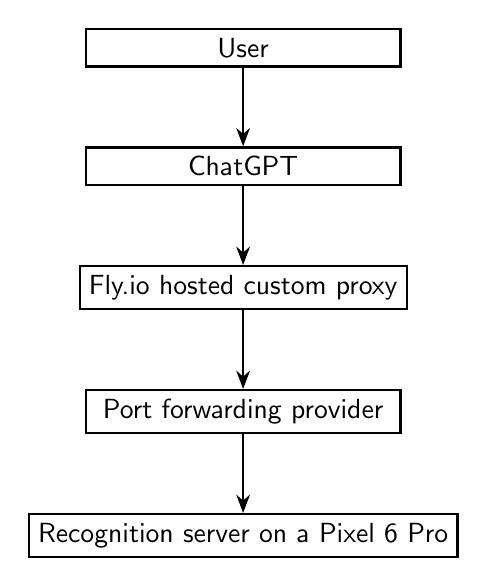
\begin{tikzpicture}[
    node distance=1cm,
    every node/.style={fill=white, font=\sffamily, draw=black, thick, align=center, minimum width=4cm},
    every path/.style={draw, thick, -Stealth}
]

% Nodes
\node (user) {User};
\node[below=of user] (chatgpt) {ChatGPT};
\node[below=of chatgpt] (proxy) {Fly.io hosted custom proxy};
\node[below=of proxy] (port) {Port forwarding provider};
\node[below=of port] (server) {Recognition server on a Pixel 6 Pro};

% Paths
\draw (user) -- (chatgpt);
\draw (chatgpt) -- (proxy);
\draw (proxy) -- (port);
\draw (port) -- (server);

\end{tikzpicture}
\caption{Communication Flow from ChatGPT to the Recognition Server.}
\end{figure}

\end{minipage}

\subsection{Image Text Detection: Successful Meme detection}
The chosen \href{https://developers.google.com/android/reference/com/google/mlkit/vision/text/TextRecognizer}{library} worked well on our screenshots of Mastodon memes, completing the detection in under a second. This detection consumed no water (unlike commercial operators \cite{li2023making}) and was powered by our personal solar panel so caused no scope 1 CO2 emissions\cite{world2004greenhouse}. It also fulfilled our data residency requirements, as the text detection was performed in our residence's living room. The fact the images got sent to OpenAI first, and via an intermediary, should be ignored.

\section{Results: Missing Data}
While we convinced the GPT that our server exists, and that it has an API worthy of its use, we entirely failed to get it to send any image provided. It preferred to send empty request bodies regardless of how many riches offered or penalties threatened.
From this we inferred that this multimodal GPT doesn't actually understand images, and there's some supporting middleware that displays the images when the model wants to present them, rather than them being in the context in full.
Some others had some luck tricking the GPT in order to send their files, mostly via base64 encoding but we were not so fortunate\cite{OpenAICommunity2024}.

\section{Discussion: Were We Mad To Try This?}
Yes. Yes, we were. It became abundantly clear that expecting current multi-modal GPT models to understand and interpret images on local hardware was like expecting a tractor to be able to drive through Camden market.

\section{Conclusions: A Reflection on Our Overambitious Dreams}
This investigation into the application of multi-modal GPT models for image text detection on local hardware was a fun failed experiment. Our conclusion — that current models lack a true understanding of images — is a testament to our excessive imagination and underwhelming execution. We await the day when more advanced models emerge, models that do not just see images but understand them, embracing their complexity with the grace of a thousand bees. Until then, we recommend doing text recognition the old fashioned way, with our eyes.


\section*{Acknowledgements}
The author would like to express their gratitude to several individuals and machines who made this research possible:

\begin{itemize}
    \item Diana Licheva, for her patience and dry humour throughout the research process.
    \item The reviewer(s) for skimming through this nonsense.
    \item ChatGPT, for making it far faster to create a LaTeX document, for generating a template and for giving this research a reason to exist.
    \item The kettle, for providing hot water for tea every time it was required.
    
\end{itemize}

\begin{sloppypar} % to force the URLs to fit on the page
\printbibliography 
\end{sloppypar}

\end{document}
